\documentclass[10pt,twocolumn,a4paper]{article}
\usepackage[margin=18mm,columnsep=6mm]{geometry}
\usepackage{amsmath,amssymb,booktabs,microtype,graphicx,tikz,pgfplots}
\usepackage[hidelinks]{hyperref}
\usepackage{xurl,placeins}
\pgfplotsset{compat=1.18}
\setlength{\emergencystretch}{1em}
\newsavebox{\databox}
\renewcommand{\dbltopfraction}{.9}
\renewcommand{\textfraction}{.1}
\title{Digital-Twin-Guided Predictive Autoscaling:\\Capacity Calibration, Ready Reserves and Repeated Kubernetes Evaluation}
\author{Shehryar Faisal}
\date{November 2026}
\renewcommand{\dbltopfraction}{0.95}
\renewcommand{\dblfloatpagefraction}{0.85}
\renewcommand{\textfraction}{0.05}
\begin{document}
\twocolumn[\begin{@twocolumnfalse}\maketitle
\begin{abstract}
Predictive autoscaling can fail when forecast uncertainty, service capacity and replica readiness are treated separately. We preserve a published Prophet--LSTM reproduction and investigate why an initial latency-Twin controller met a strict request objective inconsistently. A revised controller replaces an absolute latency-error correction with a measured capacity envelope, a conservative demand bound, recent CPU-cost information, ready capacity reserves and guarded scale-down. Development measurements showed that fixed six-replica capacity failed at peak conditions on the current host, motivating a shared sixteen-replica maximum for the expanded comparison. We execute 75 primary Kubernetes trials across five policies, five repetitions and three workloads, plus eighteen reserve-matched follow-up trials, eighteen independent response-validation blocks and 1,000 independent-plant rollouts.

The primary cohort measures 120275 requests. The revised controller meets the 99\% HTTP-success-within-500-ms objective in 15 of 15 trials, compared with 0 for the original dual policy and 1 for CPU HPA. Mean trial violation rates are 0.00\%, 19.82\% and 31.65\%, respectively. The revised controller uses 27.99 mean desired pod-minutes versus 34.18 for fixed sixteen-replica capacity. Reserve-matched HPA complies in 9 of nine follow-up cells, qualifying attribution of the primary gain. These finite results characterize a reliability--allocation tradeoff on one local service; they do not certify a general SLO guarantee. Code and experimental artifacts are available at \url{https://github.com/shehryarf67/uncertainty-aware-digital-twin-k8s-autoscaling}.\end{abstract}\vspace{4mm}\end{@twocolumnfalse}]


\section{Introduction}
Kubernetes autoscaling observes demand and resource use, then requests capacity that becomes useful only after replicas are ready. CPU-based Horizontal Pod Autoscaling (HPA) and KEDA provide established execution mechanisms \cite{j01,j02}. A forecast alone does not determine the resources needed for a latency objective. Request cost, CPU throttling, routing and readiness affect the demand-to-performance relationship.

Our research began with the Prophet--LSTM approach of Guruge and Priyadarshana \cite{guruge}. We first reproduced the released calculations and implemented a separate causal evaluation. An initial uncertainty-aware service-response Twin then exposed two practical failures: sudden demand reached the application before scale-up completed, and large absolute latency residuals made every surrogate replica choice infeasible. Simply adding a larger latency margin did not establish request-level compliance.

This article studies an implemented repair rather than claiming a new general class of autoscaling. We calibrate a service-capacity envelope from development measurements, retain ready capacity, react conservatively to observed pressure, and restrict scale-down while the observed violation fraction is high. We compare this controller with the original dual policy under a common expanded capacity limit, a reserve ablation, native CPU HPA and a fixed-capacity reference. Previous results remain available as a diagnostic pilot, not a resource-matched estimate of the revision's effect.

We ask: (RQ1) what does a faithful forecasting reproduction establish after causal evaluation; (RQ2) how consistently does the revision meet the measured SLO, and at what allocation cost; and (RQ3) which roles do reserve capacity, pressure response and planning horizon play under bursts, drift and observation or startup delay? The evidence combines saved historical forecasts, repeated real Kubernetes execution and a separate queueing plant. Each has a distinct scope.

\section{Related Work}
Prophet models trend and seasonal structure \cite{prophet}; LSTM provides gated recurrent memory \cite{lstm}. The reference hybrid assigns trend and seasonality to Prophet and forecasts residuals with an LSTM \cite{guruge}. Our neural reproduction concerns this baseline, while the live controller uses a lightweight short-horizon predictor so that policy differences are not confused with retraining a larger forecaster.

Research surveys cover cloud elasticity, container scaling and edge or IoT settings \cite{j06,j08,j09,j24,j26}. Kubernetes studies examine HPA operation, tuning, workload prediction and SLA-aware thresholds \cite{j01,j02,j03,j04}. Their differing workloads and settings make cross-paper numerical rankings unreliable.

Predictive studies use recurrent, transformer and other workload models in container and cloud resource management \cite{j05,j13,j15,j16,j18,j22,j23,j25,j29}. Other journal studies consider adaptive containers, bio-inspired scaling, online virtual-machine scaling, multi-resource neural control and dynamic workloads \cite{j07,j10,j11,j14,j17}. Capacity-transition costs and formal correctness have also been studied \cite{j12,j27}.

Digital-twin architectures describe broader physical--virtual synchronization and lifecycle concerns \cite{j19,j28}. Our implemented service-response model addresses only a restricted conditional mapping. Related conformal time-series work studies multi-step prediction intervals \cite{j20,j21}; the revision's finite-window maximum-score correction does not inherit these methods' guarantees. Workload-bound coverage and request-level latency compliance are different events. The contribution is an auditable empirical study of concrete failure repairs and their costs, not a claim to establish a new general class of autoscaling.

\section{Baseline Validation}
Let $y_t$ be workload, $p_t$ a Prophet estimate and $r_t=y_t-p_t$ its residual. A causal one-minute hybrid predicts
\begin{equation}\widehat y_{t\mid t-1}=p_t+f_\theta(r_{t-1}).\end{equation}
The scored observation is excluded from its input. Earlier observed test counts may enter later forecasts: this is rolling one-step evaluation. The official supplied NASA-HTTP and WorldCup98 files contain 81,396 and 125,300 observed minute rows, with chronological 70/30 partitions of 56,977/24,419 and 87,710/37,590. They omit 7,884 and ten calendar minutes. Gap filtering leaves 24,390 NASA and 37,590 WorldCup eligible targets; missing traffic is not asserted to be zero.

The main released notebooks use linear Prophet growth for NASA and flat growth for WorldCup, changepoint prior 5.1, seasonality prior 30, daily/weekly Fourier orders 50/20 and no yearly seasonality. Two 50-unit LSTM layers and a linear output use look-back one, Adam/MSE, batch 16, a 20-epoch cap, validation fraction 0.2 and patience-five early stopping with restored best weights. The article prints 50 epochs. Four faithful fits, two per dataset, stop after six epochs and restore epoch-one weights. The CPU environment uses Python 3.12.14, TensorFlow 2.17, Keras 3.4.1 and Prophet 1.1.5 on an Intel i7-1255U.

The released combination places a next-row residual prediction on the current row and fills its final missing prediction with observed truth. NASA residual scaling and WorldCup count scaling include test data. Faithful runs retain these behaviours. A separate implementation fixes alignment and the truth fallback, fits transforms on the early neural fitting prefix, filters gaps and fixes random states to 42. Prophet fits the full outer training period; neural validation is conditional on that fitted Prophet, while outer-test observations remain outside fitting. The changes are joint corrections, not a one-factor ablation.


\begin{table}[t]\centering\small\setlength{\tabcolsep}{3pt}
\caption{Forecast RMSE. Faithful means use full released tests; causal NASA excludes 29 gap targets. WorldCup is displayed on the common author scale after causal fitting.}\label{tab:baseline}
\savebox{\databox}{%
\begin{tabular}{lrrr}\toprule
Trace & Published & Faithful & Causal\\\midrule
NASA & 7.990 & 8.02163 & 14.2902\\
WorldCup & 0.003358 & 0.00337950 & 0.00388174\\
\bottomrule\end{tabular}
}
\ifdim\wd\databox>\columnwidth\relax\resizebox{\columnwidth}{!}{\usebox{\databox}}\else\usebox{\databox}\fi
\end{table}


On common NASA targets, faithful mean RMSE is 8.01251. WorldCup causal raw-count RMSE is 890.5685, compared with persistence at 762.7463; NASA persistence is 16.3871. The higher causal errors change the interpretation of the released scores without identifying one isolated cause. Original models, predictions and inputs are preserved.

\section{Initial Controller Diagnosis}
An earlier integration check connected the authors' Java 21/Spring Boot 3.4.2 application and forecasting scaler to KEDA 2.18, Prometheus 2.55.1 and local K3s. Scaler logic was preserved while compatible gRPC bindings were regenerated. Stable, increasing, spike and decreasing scenarios produced 6,870 measured requests per controller in scheduling-validated runs. Forecast KEDA and CPU HPA had zero HTTP failures and zero observations above 500 ms. Forecast scaling held three replicas; HPA moved from one to three. Sampled allocation was 23.286 versus 13.778 pod-minutes. These short integration sequences established actuation without exposing a useful overload boundary.

The subsequent CPU-service pilot fitted a monotone effective-P99 response Twin, $g(x)$, to $x=\lambda c/n$, where $\lambda$ is offered rate, $c$ median CPU milliseconds and $n$ ready replicas. Eighteen fit and twelve calibration blocks initialized a frozen curve and a separate latency residual margin. The policy combined this with a demand residual margin, planning over two cycles and enumerating one to six replicas. Each cycle offered five seconds of traffic and reserved three seconds for drainage.

Across fifteen pilot trials, the dual policy averaged 10.40\% request violations and satisfied the strict SLO in only one of three repetitions. Point-Twin control averaged 39.67\%. Twelve of 48 dual decisions carried a latency correction above the 500-ms target itself, making every positive-latency candidate fail its surrogate constraint. Maximum-replica fallback was therefore not evidence of feasible constraint satisfaction. Conditional mapping residuals also mixed queueing under the realized state with the counterfactual effect of adding capacity. These observations motivated the revision.

\section{Controller Revision}
\subsection{Objective and Capacity Evidence}
A request complies only if HTTP status is 200 and measured client latency $\ell_i\leq500$ ms. The request objective is
\begin{equation}v=\frac{1}{N}\sum_i\mathbf1\{\mathrm{status}_i\ne200\lor\ell_i>500\mathrm{\ ms}\}\leq0.01.\label{eq:slo}\end{equation}
Timeouts and fast rejections count as violations. This objective differs from workload prediction coverage. Allocation is desired-replica pod-minutes, including pending capacity, rather than monetary billing or CPU energy.

We retain the same instrumented PBKDF2 CPU service. A pod requests 250m CPU/96Mi and is limited to 500m/192Mi. A single processing semaphore serializes work per pod; queue waits beyond two seconds return HTTP 429 and clients time out after three seconds. Readiness includes a five-second startup delay and two-second probe cadence. Kubernetes CPU limits can impose throttling \cite{j01,j12}. The author application and original baseline files are unchanged.

Before final testing, development capacity measurements cross four offered-load/work conditions with 4, 6, 8, 12 and 16 fixed replicas. Conditions are 5, 25 and 45 requests/s with unit work, and 30 requests/s with 1.8-fold work. The 4--12-replica blocks use five seconds of offered traffic and three seconds of drainage; sixteen-replica blocks extend offered traffic to fifteen seconds. These twenty blocks contain 3,675 measured requests. At the current host conditions, fixed six replicas failed the target at peak traffic and higher work cost; sixteen had no observed violations in the longer checks. This is empirical capacity evidence, not a proof that every six-replica strategy is impossible. The expanded comparison consequently gives every adaptive policy the same sixteen-replica ceiling.

For development block $j$, define $x_j=\lambda_jc_j/n_j$. A monotone response curve is fitted to measured effective P99. For model diagnostics, a failure receives an effective penalty of at least 2,000 ms so that fast errors do not resemble good service. Actual SLO metrics and client quantiles always use measured latency and status. Sizing uses an operating envelope extracted from the same development profile:
\begin{align}
\mathcal A&=\{j:v_j\leq0.01,\ P99_j\leq400\mathrm{\ ms}\},\\
C&=\min\{200,\ 0.8\max_{j\in\mathcal A}x_j\}.\label{eq:capacity}
\end{align}
The 20\% headroom and 400-ms screening target are engineering choices fixed before evaluation. $C$ is CPU milliseconds per second per ready replica; it is not a confidence-certified capacity estimate. The frozen response curve supplies support and tail diagnostics, while this empirical envelope directly drives replica sizing.

\subsection{Demand and Cost Corrections}
The controller observes completed outcomes, issued-request counts and current replica state. Initial rate history uses two measured five-RPS warm-up cycles. Initial CPU cost uses their successful-response P90. A rolling maximum of the most recent four available response CPU-P90 estimates provides $\bar c_t$, allowing immediate upward adjustment and slower decay after a service-cost shift. Failed or incomplete responses do not reveal future CPU work.

For horizon $h_t$, the point demand forecast is the maximum of the last three observed rates and the current rate extrapolated using the latest nonnegative rate increase. Forecast errors compare an issued point with the maximum of the next $h_t$ observed rates. An error enters calibration only after its full horizon matures. The last forty signed errors provide a nonnegative nominal-99\% upper correction $q_t$, with finite ranks capped at the largest observed score. With at most forty scores, this maximum-score rule does not provide exact distribution-free 99\% finite-sample coverage. We evaluate it empirically and make no inherited conformal guarantee.

\subsection{Readiness, Pressure and Scale-Down}
Observed desired-to-ready transitions update a startup estimate using equal weight on its previous value and the latest observed transition lag, floored at eight seconds. The horizon is
\begin{equation}h_t=\max\{2,\min(6,\lceil\widehat d_t/8\rceil+1)\}.\end{equation}
The nominal startup estimate is eight seconds. At each completed observation, the provisional replica requirement is
\begin{equation}n_t^{\rm req}=\left\lceil\frac{(\widehat\lambda_t+q_t)\bar c_t}{C\beta_t}\right\rceil+2,\label{eq:sizing}\end{equation}
clipped to the common maximum, with an eight-replica desired reserve initialized with all eight ready. The two additional replicas and reserve are explicit resource costs. The reserve ablation removes only the eight-replica floor; it begins with the same eight ready replicas and retains the other logic.

The factor $\beta_t\in[0.5,1]$ tightens by a factor 0.85 when observed violations exceed 0.5\% or effective P99 exceeds 450 ms. After eight clean observations it recovers by 0.025 per cycle, up to one. Violations above 1\%, effective P99 above 500 ms, or an active three-cycle pressure hold request the maximum. Scale-down requires three lower recommendations, three clean observations, no ready deficit and cumulative observed violations at most 0.5\%. At most one replica is removed per decision. This is a conservative burn guard rather than a general budget-pacing optimizer.

Unsupported or over-limit demand is logged. Neither a maximum-capacity request nor a diagnostic ``feasible'' flag proves Equation~\ref{eq:slo}. The revision avoids applying an irreducible absolute latency residual to every counterfactual replica count, but still relies on approximate balancing, finite profiling and service instrumentation.

\begin{figure}[t]\centering
\resizebox{\columnwidth}{!}{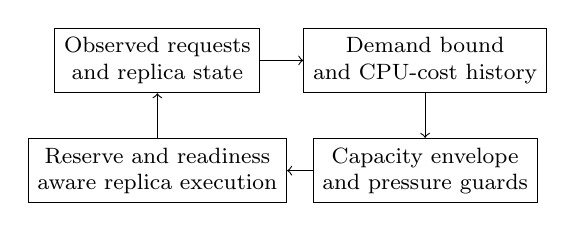
\begin{tikzpicture}[font=\footnotesize]
\node[draw,align=center] (o) at (0,0) {Observed requests\\and replica state};
\node[draw,align=center] (p) at (3.4,0) {Demand bound\\and CPU-cost history};
\node[draw,align=center] (t) at (3.4,-1.4) {Capacity envelope\\and pressure guards};
\node[draw,align=center] (a) at (0,-1.4) {Reserve and readiness\\aware replica execution};
\draw[->] (o)--(p);\draw[->] (p)--(t);\draw[->] (t)--(a);\draw[->] (a)--(o);
\end{tikzpicture}}
\caption{Implemented revision. Decisions use only observed telemetry; future traffic and work schedules remain confined to the load generator.}\label{fig:architecture}\end{figure}

\section{Experimental Design}
\subsection{Repeated Kubernetes Evaluation}
The cluster remains K3s v1.33.6+k3s1/containerd 2.1.5 under Ubuntu WSL2 on the local Intel CPU host. A loopback-only API proxy serves the external controller. Source, development inputs and controller settings are hashed before final comparisons. Existing forecasting and pilot artifacts remain preserved.

Five policies are tested: guarded revision, original dual policy, reserve ablation, native CPU HPA and fixed sixteen replicas. The original dual algorithm and its earlier fitted profile are retained; its replica maximum is raised to sixteen for this comparison. All adaptive policies start with eight ready replicas. The fixed reference is provisioned with sixteen before measurement, so it is a capacity/cost reference with an explicit initial-capacity advantage. Two common low-rate warm-up cycles and setup allocation are excluded. Results concern the measured trial interval, not full deployment lifetime billing.

Native HPA uses a 70\% CPU-request target, replica bounds one to sixteen, zero scale-up stabilization and a 24-second scale-down stabilization window. It is installed after warm-up to preserve the common initial adaptive capacity. HPA retains native reconciliation and sensing timing \cite{j01}; external policies decide every eight seconds. This is an operational comparison, not a timing-matched implementation of the same algorithm.

An exploratory follow-up addresses minimum-replica confounding directly. It compares the unchanged guarded controller with native HPA whose minimum is also eight and maximum sixteen. Three fresh seeds, 909, 1010 and 1111, give eighteen additional trials across the same three workloads, with randomized within-seed policy and scenario ordering. This follow-up was specified after early primary outcomes had been inspected; its paired results are reported separately rather than being portrayed as part of the original frozen 75-comparison plan. No controller parameters are refitted.

Seeds 404, 505, 606, 707 and 808 define five repetitions. Scenario and policy orders are shuffled deterministically per seed. The three sixteen-cycle workloads are fixed before final testing (Table~\ref{tab:workloads}). The previous batch shape is deliberately reused and is not claimed to be an unseen workload. Two new shapes introduce abrupt changes or uninterrupted traffic. The controller never receives their future rates or work multipliers.


\begin{table*}[t]\centering\small\setlength{\tabcolsep}{3pt}
\caption{Each cycle spans eight seconds. Batch workloads offer traffic for five seconds and pause for three; continuous traffic uses all eight. Work multipliers rise to 1.8 in cycles 13--16 of the previous batch, to 1.6 in cycles 11--13 of abrupt batch, and to 1.6 in cycles 11--16 of continuous traffic. Other cycles use unit work.}\label{tab:workloads}
\savebox{\databox}{%
\begin{tabular}{lrrl}\toprule
Workload & Active s/cycle & Requests/trial & Rate sequence (requests/s)\\\midrule
Previous batch & 5 & 1400 & 5, 5, 5, 5, 10, 15, 20, 25, 45, 45, 15, 10, 25, 30, 15, 5\\
Abrupt batch & 5 & 1315 & 5, 5, 5, 5, 40, 40, 40, 8, 8, 8, 28, 28, 28, 5, 5, 5\\
Continuous & 8 & 2096 & 6, 6, 9, 15, 22, 32, 40, 18, 8, 5, 25, 30, 18, 8, 15, 5\\
\bottomrule\end{tabular}
}
\ifdim\wd\databox>\textwidth\relax\resizebox{\textwidth}{!}{\usebox{\databox}}\else\usebox{\databox}\fi
\end{table*}


The generator uses absolute send deadlines, jittered request slots and no connection reuse. Traffic production runs independently of telemetry and control, preventing controller API time from creating artificial drain pauses in continuous trials. Requests retain send/finish times, HTTP status, latency, CPU and queue information where observed, and dispatch delay. Every scheduled request enters final scoring, including late completions and timeouts. Control feedback at a boundary uses completed outcomes before that boundary and outstanding-response ages, with no future response payloads.

An independent sampler records desired and ready replicas approximately once per second. Desired pod-minutes integrate these observations with the measured terminal partial interval. The audit independently bounds the terminal contribution because its exact terminal clock is not separately archived. Dispatch delay must remain below 500 ms, sampler gaps below three seconds, decision lateness below one second, and request counts must match the schedule. A timing-invalid attempt may be repeated once; all attempts remain available. SLO failures are valid outcomes and never trigger replacement.

\subsection{Historical Bounds and Independent Plant}
Saved causal forecasts are evaluated without retraining weights. The first 20\% of previously eligible outer-test targets form a new calibration prefix: 4,878 NASA and 7,518 WorldCup observations. Remaining rolling evaluations contain 19,512 and 30,072 targets. Static calibration uses the prefix's upper-error quantile; adaptive calibration starts from its last forty errors and updates after each outcome. These trace-bound results concern demand events, not request-latency certification.

Independent response validation uses eighteen new combinations: fixed replica counts 6, 10 and 14; rates 12, 24 and 36 requests/s; and work multipliers 1.1 and 1.5. Each has five seconds of offered load and three seconds of drainage, producing 2,160 additional measured requests. Neither the response curve nor operating envelope is refitted. CPU input for this check is realized within the block, so it validates the conditional response mapping, not ex-ante CPU forecasting or a full-cluster counterfactual guarantee.

The new simulator generates labels using Poisson arrivals and independent lognormal CPU work, never using the fitted response Twin. Log-scale standard deviation is 0.3 and mean CPU work derives from unit-work development measurements. A central dispatcher assigns requests to the earliest free ready server supplying 0.5 CPU core. Queue admission and three-second client timeout are modeled; successful completed responses alone expose their CPU work. Removed-server outcomes remain scored.

Twenty-five paired seeds, five regimes and eight policies give 1,000 rollouts of 64 eight-second cycles. Regimes cover smooth demand, bursts, a 1.8-fold service-cost shift, startup delay increased from eight to 24 seconds, and one-cycle observation delay. In the delay case, demand, response and CPU feedback are delayed while replica state remains current. Policies include the guarded revision, reserve ablation, original dual policy, CPU-reactive proxy, fixed eight and fixed sixteen replicas, and isolated emergency-response and horizon ablations. The latter change only the named assignment in the frozen controller method. The proxy is not native HPA. Shared arrival/service input hashes verify pairing across policies.

\subsection{Analysis and Claim Scope}
We report per-workload compliance counts, mean trial violation rates, mean per-trial P99 and allocation. Paired seed differences compare the revision with each live comparator. Descriptive percentile bootstrap intervals use 10,000 resamples of the five paired repetitions \cite{bootstrap}. Requests within a run are temporally dependent and are not treated as independent statistical replications. With five repetitions, interval precision is limited; an all-zero empirical outcome can yield a degenerate bootstrap interval without proving zero risk. Simulation intervals characterize the selected plant and seeds rather than a population of real clusters.

\section{Results}
\subsection{Preserved Forecasting Evidence}


\begin{table}[t]\centering\small\setlength{\tabcolsep}{3pt}
\caption{Held-out historical demand upper-bound coverage (\%), nominal 90\%. This analysis uses a new calibration prefix of saved test predictions and does not change predictor weights.}\label{tab:historical}
\savebox{\databox}{%
\begin{tabular}{lrrr}\toprule
Trace & Point & Static & Adaptive\\\midrule
NASA & 57.52 & 89.74 & 90.02\\
WorldCup & 78.87 & 96.87 & 90.33\\
\bottomrule\end{tabular}
}
\ifdim\wd\databox>\columnwidth\relax\resizebox{\columnwidth}{!}{\usebox{\databox}}\else\usebox{\databox}\fi
\end{table}

The adaptive historical bounds approach their nominal workload coverage. WorldCup static bounds are more conservative. This does not reduce point forecast RMSE or imply that the later control loops achieve their request SLO.
\subsection{Development Capacity Checks}

\begin{table*}[t]\centering\small\setlength{\tabcolsep}{3pt}
\caption{Development measurements preceding final tests. These are single blocks per condition; sixteen-replica offered-load blocks last fifteen seconds, other blocks five. Sampling variability and host conditions limit the inferred capacity boundary.}\label{tab:capacity}
\savebox{\databox}{%
\begin{tabular}{lrrrr}\toprule
Replicas & 45 RPS bad \% & P99 ms & 30 RPS, 1.8 work bad \% & P99 ms\\\midrule
4 & 66.67 & 1672.96 & 82.67 & 2125.10\\
6 & 13.33 & 1573.10 & 18.67 & 1107.37\\
8 & 0.00 & 418.88 & 18.67 & 1114.10\\
12 & 0.00 & 195.61 & 0.67 & 456.99\\
16 & 0.00 & 182.59 & 0.00 & 405.60\\
\bottomrule\end{tabular}
}
\ifdim\wd\databox>\textwidth\relax\resizebox{\textwidth}{!}{\usebox{\databox}}\else\usebox{\databox}\fi
\end{table*}

The selected operating threshold is 170.12 CPU-ms/s per ready replica. The capacity measurements justify evaluating a larger shared ceiling, while the matched reruns, rather than a direct comparison with the old six-replica pilot, assess policy differences under that ceiling.

\begin{table}[t]\centering\small\setlength{\tabcolsep}{3pt}
\caption{Independent response mapping at eighteen new load/work/replica combinations, using realized CPU input. Screening an operating point as safe is not a guarantee for future traffic.}\label{tab:fidelity}
\savebox{\databox}{%
\begin{tabular}{lr}\toprule
Conditional response check & Observed\\\midrule
Effective-P99 MAE (ms) & 94.04\\
Median absolute error (ms) & 88.45\\
SLO-compliant fixed-load blocks & 18/18\\
False-safe envelope cases & 0/17\\
\bottomrule\end{tabular}
}
\ifdim\wd\databox>\columnwidth\relax\resizebox{\columnwidth}{!}{\usebox{\databox}}\else\usebox{\databox}\fi
\end{table}

The independent validation measures 2160 requests. It evaluates interpolation to new rate/work combinations and replica counts; its conditional CPU input and one short block per condition limit ex-ante and counterfactual interpretations.

\subsection{Repeated Live SLO Outcomes}

\begin{table*}[t]\centering\small\setlength{\tabcolsep}{3pt}
\caption{Means across five real Kubernetes repetitions. P99 is the mean of per-run client P99 values. SLO runs satisfy at least 99\% HTTP-200 responses within 500 ms. Intervals resample runs; zero empirical violations do not certify zero future risk.}\label{tab:live}
\savebox{\databox}{%
\begin{tabular}{lllrrrr}\toprule
Workload & Policy & Met & Bad \% & 95\% interval & P99 ms & Pod-min\\\midrule
Previous batch & Guarded Twin & 5/5 & 0.00 & [0.00, 0.00] & 146.09 & 26.53\\
Previous batch & Original dual & 0/5 & 7.41 & [3.09, 11.84] & 1232.23 & 20.16\\
Previous batch & No reserve & 5/5 & 0.00 & [0.00, 0.00] & 128.79 & 25.87\\
Previous batch & CPU HPA & 0/5 & 50.96 & [45.93, 58.54] & 2107.88 & 8.89\\
Previous batch & Fixed sixteen & 5/5 & 0.00 & [0.00, 0.00] & 124.14 & 34.18\\
Abrupt batch & Guarded Twin & 5/5 & 0.00 & [0.00, 0.00] & 192.91 & 28.77\\
Abrupt batch & Original dual & 0/5 & 31.39 & [30.01, 32.56] & 2101.83 & 21.78\\
Abrupt batch & No reserve & 5/5 & 0.11 & [0.03, 0.18] & 294.23 & 28.42\\
Abrupt batch & CPU HPA & 0/5 & 31.50 & [24.44, 38.56] & 1971.41 & 9.02\\
Abrupt batch & Fixed sixteen & 5/5 & 0.00 & [0.00, 0.00] & 135.84 & 34.17\\
Continuous & Guarded Twin & 5/5 & 0.00 & [0.00, 0.00] & 118.62 & 28.69\\
Continuous & Original dual & 0/5 & 20.67 & [16.71, 23.49] & 2079.83 & 26.76\\
Continuous & No reserve & 5/5 & 0.01 & [0.00, 0.03] & 126.35 & 28.95\\
Continuous & CPU HPA & 1/5 & 12.48 & [3.23, 23.56] & 1236.34 & 11.71\\
Continuous & Fixed sixteen & 5/5 & 0.00 & [0.00, 0.00] & 112.40 & 34.18\\
\bottomrule\end{tabular}
}
\ifdim\wd\databox>\textwidth\relax\resizebox{\textwidth}{!}{\usebox{\databox}}\else\usebox{\databox}\fi
\end{table*}

All 75 selected comparisons contain 120275 scored requests. 1 additional timing-invalid attempts are retained. Across the fifteen workload--seed cells, guarded control complies in 15, the original dual policy in 0, CPU HPA in 1, the reserve ablation in 15, and fixed sixteen in 15. Means across trials give 0.00\% violations for the revision versus 19.82\% for original dual control. Different workloads offer different numbers of requests; compliance counts and the per-workload table therefore remain primary, rather than substituting a pooled percentage for each trial objective.

\begin{figure*}[t]\centering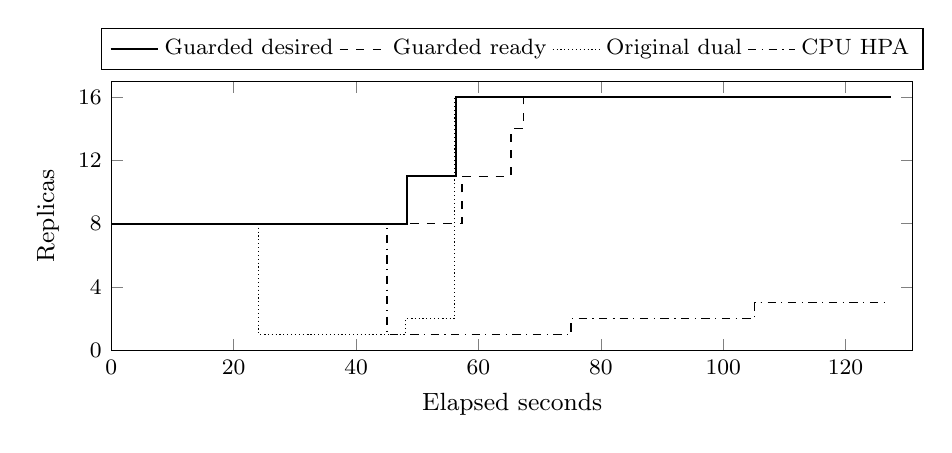
\begin{tikzpicture}\begin{axis}[width=.97\textwidth,height=5cm,xlabel={Elapsed seconds},ylabel={Replicas},xmin=0,xmax=131,ymin=0,ymax=17,ytick={0,4,8,12,16},legend style={at={(.5,1.04)},anchor=south,legend columns=4,font=\footnotesize},tick label style={font=\footnotesize},label style={font=\small}]
\addplot[const plot,no marks,black,thick] coordinates {(0.000,8) (1.001,8) (2.002,8) (3.004,8) (4.004,8) (5.005,8) (6.007,8) (7.009,8) (8.010,8) (9.011,8) (10.011,8) (11.012,8) (12.013,8) (13.014,8) (14.015,8) (15.017,8) (16.017,8) (17.018,8) (18.019,8) (19.021,8) (20.021,8) (21.023,8) (22.025,8) (23.027,8) (24.027,8) (25.028,8) (26.029,8) (27.030,8) (28.032,8) (29.033,8) (30.036,8) (31.037,8) (32.066,8) (33.066,8) (34.067,8) (35.068,8) (36.069,8) (37.070,8) (38.071,8) (39.074,8) (40.089,8) (41.089,8) (42.090,8) (43.090,8) (44.091,8) (45.092,8) (46.093,8) (47.095,8) (48.283,11) (49.284,11) (50.287,11) (51.287,11) (52.288,11) (53.290,11) (54.292,11) (55.294,11) (56.306,16) (57.307,16) (58.308,16) (59.310,16) (60.312,16) (61.313,16) (62.316,16) (63.317,16) (64.318,16) (65.319,16) (66.320,16) (67.320,16) (68.321,16) (69.323,16) (70.325,16) (71.327,16) (72.328,16) (73.330,16) (74.331,16) (75.331,16) (76.332,16) (77.333,16) (78.336,16) (79.337,16) (80.338,16) (81.340,16) (82.340,16) (83.341,16) (84.342,16) (85.343,16) (86.345,16) (87.347,16) (88.349,16) (89.351,16) (90.352,16) (91.353,16) (92.353,16) (93.354,16) (94.356,16) (95.358,16) (96.358,16) (97.359,16) (98.360,16) (99.361,16) (100.363,16) (101.365,16) (102.367,16) (103.369,16) (104.370,16) (105.370,16) (106.372,16) (107.372,16) (108.373,16) (109.374,16) (110.376,16) (111.379,16) (112.380,16) (113.381,16) (114.382,16) (115.383,16) (116.384,16) (117.385,16) (118.386,16) (119.388,16) (120.388,16) (121.389,16) (122.390,16) (123.390,16) (124.392,16) (125.393,16) (126.394,16) (127.396,16)};
\addlegendentry{Guarded desired}
\addplot[const plot,no marks,black,dashed] coordinates {(0.000,8) (1.001,8) (2.002,8) (3.004,8) (4.004,8) (5.005,8) (6.007,8) (7.009,8) (8.010,8) (9.011,8) (10.011,8) (11.012,8) (12.013,8) (13.014,8) (14.015,8) (15.017,8) (16.017,8) (17.018,8) (18.019,8) (19.021,8) (20.021,8) (21.023,8) (22.025,8) (23.027,8) (24.027,8) (25.028,8) (26.029,8) (27.030,8) (28.032,8) (29.033,8) (30.036,8) (31.037,8) (32.066,8) (33.066,8) (34.067,8) (35.068,8) (36.069,8) (37.070,8) (38.071,8) (39.074,8) (40.089,8) (41.089,8) (42.090,8) (43.090,8) (44.091,8) (45.092,8) (46.093,8) (47.095,8) (48.283,8) (49.284,8) (50.287,8) (51.287,8) (52.288,8) (53.290,8) (54.292,8) (55.294,8) (56.306,8) (57.307,11) (58.308,11) (59.310,11) (60.312,11) (61.313,11) (62.316,11) (63.317,11) (64.318,11) (65.319,14) (66.320,14) (67.320,16) (68.321,16) (69.323,16) (70.325,16) (71.327,16) (72.328,16) (73.330,16) (74.331,16) (75.331,16) (76.332,16) (77.333,16) (78.336,16) (79.337,16) (80.338,16) (81.340,16) (82.340,16) (83.341,16) (84.342,16) (85.343,16) (86.345,16) (87.347,16) (88.349,16) (89.351,16) (90.352,16) (91.353,16) (92.353,16) (93.354,16) (94.356,16) (95.358,16) (96.358,16) (97.359,16) (98.360,16) (99.361,16) (100.363,16) (101.365,16) (102.367,16) (103.369,16) (104.370,16) (105.370,16) (106.372,16) (107.372,16) (108.373,16) (109.374,16) (110.376,16) (111.379,16) (112.380,16) (113.381,16) (114.382,16) (115.383,16) (116.384,16) (117.385,16) (118.386,16) (119.388,16) (120.388,16) (121.389,16) (122.390,16) (123.390,16) (124.392,16) (125.393,16) (126.394,16) (127.396,16)};
\addlegendentry{Guarded ready}
\addplot[const plot,no marks,black,densely dotted] coordinates {(0.000,8) (1.002,8) (2.003,8) (3.004,8) (4.005,8) (5.006,8) (6.008,8) (7.011,8) (8.023,8) (9.023,8) (10.025,8) (11.025,8) (12.026,8) (13.027,8) (14.029,8) (15.030,8) (16.031,8) (17.032,8) (18.034,8) (19.036,8) (20.037,8) (21.039,8) (22.040,8) (23.042,8) (24.043,1) (25.043,1) (26.044,1) (27.045,1) (28.046,1) (29.047,1) (30.048,1) (31.051,1) (32.066,1) (33.066,1) (34.066,1) (35.067,1) (36.068,1) (37.070,1) (38.071,1) (39.072,1) (40.072,1) (41.074,1) (42.074,1) (43.075,1) (44.075,1) (45.076,1) (46.077,1) (47.079,1) (48.125,2) (49.125,2) (50.126,2) (51.126,2) (52.127,2) (53.128,2) (54.128,2) (55.130,2) (56.132,16) (57.133,16) (58.138,16) (59.140,16) (60.142,16) (61.142,16) (62.143,16) (63.145,16) (64.148,16) (65.149,16) (66.149,16) (67.150,16) (68.152,16) (69.153,16) (70.155,16) (71.156,16) (72.157,16) (73.158,16) (74.158,16) (75.159,16) (76.159,16) (77.160,16) (78.162,16) (79.164,16) (80.165,16) (81.166,16) (82.166,16) (83.167,16) (84.168,16) (85.169,16) (86.172,16) (87.174,16) (88.175,16) (89.177,16) (90.178,16) (91.179,16) (92.180,16) (93.181,16) (94.182,16) (95.184,16) (96.185,16) (97.187,16) (98.188,16) (99.188,16) (100.189,16) (101.190,16) (102.193,16) (103.196,16) (104.196,16) (105.197,16) (106.199,16) (107.200,16) (108.200,16) (109.201,16) (110.204,16) (111.207,16) (112.208,16) (113.209,16) (114.211,16) (115.212,16) (116.212,16) (117.213,16) (118.215,16) (119.216,16) (120.216,16) (121.216,16) (122.218,16) (123.218,16) (124.219,16) (125.220,16) (126.223,16) (127.225,16)};
\addlegendentry{Original dual}
\addplot[const plot,no marks,black,dashdotted] coordinates {(0.000,8) (1.001,8) (2.001,8) (3.002,8) (4.003,8) (5.004,8) (6.006,8) (7.007,8) (8.007,8) (9.008,8) (10.009,8) (11.010,8) (12.010,8) (13.011,8) (14.013,8) (15.015,8) (16.015,8) (17.017,8) (18.018,8) (19.018,8) (20.019,8) (21.021,8) (22.023,8) (23.026,8) (24.027,8) (25.027,8) (26.028,8) (27.029,8) (28.032,8) (29.032,8) (30.033,8) (31.035,8) (32.036,8) (33.038,8) (34.038,8) (35.039,8) (36.040,8) (37.041,8) (38.043,8) (39.044,8) (40.045,8) (41.046,8) (42.047,8) (43.048,8) (44.048,8) (45.049,1) (46.052,1) (47.055,1) (48.055,1) (49.056,1) (50.059,1) (51.059,1) (52.060,1) (53.061,1) (54.062,1) (55.063,1) (56.104,1) (57.105,1) (58.106,1) (59.106,1) (60.107,1) (61.108,1) (62.109,1) (63.110,1) (64.112,1) (65.113,1) (66.113,1) (67.117,1) (68.119,1) (69.120,1) (70.121,1) (71.123,1) (72.124,1) (73.125,1) (74.125,1) (75.128,2) (76.128,2) (77.129,2) (78.130,2) (79.131,2) (80.132,2) (81.132,2) (82.134,2) (83.135,2) (84.136,2) (85.137,2) (86.138,2) (87.140,2) (88.141,2) (89.143,2) (90.144,2) (91.144,2) (92.145,2) (93.146,2) (94.147,2) (95.150,2) (96.155,2) (97.156,2) (98.156,2) (99.158,2) (100.159,2) (101.160,2) (102.161,2) (103.163,2) (104.163,2) (105.164,3) (106.165,3) (107.166,3) (108.167,3) (109.168,3) (110.169,3) (111.170,3) (112.172,3) (113.173,3) (114.174,3) (115.175,3) (116.176,3) (117.178,3) (118.180,3) (119.181,3) (120.183,3) (121.184,3) (122.184,3) (123.185,3) (124.186,3) (125.188,3) (126.190,3) (127.192,3)};
\addlegendentry{CPU HPA}
\end{axis}\end{tikzpicture}\caption{Independent one-second replica observations from the predeclared first seed and previously used batch pattern. Desired capacity and ready capacity differ during actuation. All five repetitions enter the results; this trajectory is not selected for best SLO performance.}\label{fig:trajectory}\end{figure*}

\subsection{Allocation and Paired Comparisons}

\begin{table*}[t]\centering\small\setlength{\tabcolsep}{3pt}
\caption{Guarded minus reference comparisons over matched workload seeds. Negative violation differences favour guarded control; negative allocation changes mean fewer desired pod-minutes. References share the sixteen-replica ceiling; fixed capacity starts at sixteen.}\label{tab:paired}
\savebox{\databox}{%
\begin{tabular}{llrrr}\toprule
Workload & Reference & Bad-rate difference pp & Paired 95\% interval & Allocation change \%\\\midrule
Previous batch & Original dual & -7.41 & [-11.84, -3.09] & 31.60\\
Previous batch & CPU HPA & -50.96 & [-58.94, -45.93] & 198.48\\
Previous batch & Fixed sixteen & 0.00 & [0.00, 0.00] & -22.40\\
Abrupt batch & Original dual & -31.39 & [-32.58, -30.01] & 32.10\\
Abrupt batch & CPU HPA & -31.50 & [-38.56, -24.44] & 218.83\\
Abrupt batch & Fixed sixteen & 0.00 & [0.00, 0.00] & -15.80\\
Continuous & Original dual & -20.67 & [-23.31, -16.62] & 7.22\\
Continuous & CPU HPA & -12.48 & [-23.98, -3.23] & 144.97\\
Continuous & Fixed sixteen & 0.00 & [0.00, 0.00] & -16.06\\
\bottomrule\end{tabular}
}
\ifdim\wd\databox>\textwidth\relax\resizebox{\textwidth}{!}{\usebox{\databox}}\else\usebox{\databox}\fi
\end{table*}

Mean desired allocation is 27.99 pod-minutes for guarded control, 22.90 for the original dual policy and 34.18 for fixed sixteen. The guarded-versus-fixed difference is -18.09\%. More replicas can buy reliability; the comparison does not justify claiming simultaneous universal cost and latency improvement. Setup, warm-up and full-day idle capacity are outside these trial costs.

\subsection{Reserve-Matched Native HPA}

\begin{table*}[t]\centering\small\setlength{\tabcolsep}{3pt}
\caption{Separate exploratory cohort with both adaptive policies initialized at eight and constrained to the same minimum eight and maximum sixteen. Three fresh paired repeats per workload; the frozen primary cohort is unchanged.}\label{tab:reserve_hpa}
\savebox{\databox}{%
\begin{tabular}{lrrrrrr}\toprule
Workload & Guarded met & HPA-eight met & Guarded bad \% & HPA-eight bad \% & Guarded pod-min & HPA-eight pod-min\\\midrule
Previous batch & 3/3 & 3/3 & 0.00 & 0.00 & 26.24 & 17.09\\
Abrupt batch & 3/3 & 3/3 & 0.00 & 0.00 & 28.83 & 17.08\\
Continuous & 3/3 & 3/3 & 0.00 & 0.00 & 29.15 & 17.09\\
\bottomrule\end{tabular}
}
\ifdim\wd\databox>\textwidth\relax\resizebox{\textwidth}{!}{\usebox{\databox}}\else\usebox{\databox}\fi
\end{table*}

The reserve-matched follow-up contains 28866 requests. Guarded control complies in 9 of nine cells and minimum-eight HPA in 9. Mean allocation is 28.07 versus 17.09 pod-minutes. This comparison tests whether the primary gain over minimum-one HPA extends beyond warm capacity; it is a separate exploratory cohort rather than a retroactively randomized part of the original study.

The simpler reserve-matched HPA matches or exceeds the guarded policy in empirical compliance and uses fewer replicas. The evidence therefore does not support attributing a reliability advantage to the added forecasting/Twin logic over this stronger reference. Warm capacity is an important explanation for the primary comparison.

\subsection{Ablation and Stress Sensitivity}

\begin{table}[t]\centering\small\setlength{\tabcolsep}{3pt}
\caption{Live reserve ablation: guarded minus otherwise identical policy without the eight-replica floor. Both begin with eight ready replicas.}\label{tab:ablation}
\savebox{\databox}{%
\begin{tabular}{lrrr}\toprule
Workload & $\Delta$ bad pp & 95\% interval & $\Delta$ cost \%\\\midrule
Previous batch & 0.00 & [0.00, 0.00] & 2.53\\
Abrupt batch & -0.11 & [-0.18, -0.03] & 1.24\\
Continuous & -0.01 & [-0.03, 0.00] & -0.90\\
\bottomrule\end{tabular}
}
\ifdim\wd\databox>\columnwidth\relax\resizebox{\columnwidth}{!}{\usebox{\databox}}\else\usebox{\databox}\fi
\end{table}

The reserve ablation quantifies a specific resource-protection choice. Its observed effect varies by workload and should not be treated as a universal advantage for a fixed eight-replica floor.

\begin{table}[t]\centering\small\setlength{\tabcolsep}{3pt}
\caption{Independent-plant means across 25 paired seeds per regime. All ablation columns show violation percentages. The central queue omits Kubernetes routing and CFS details, so these values are not live-cluster outcomes. Full eight-policy scores are retained in the artifact.}\label{tab:simulation}
\savebox{\databox}{%
\begin{tabular}{lrrrrrr}\toprule
Regime & Guarded & No reserve & No emergency & $h=1$ & CPU proxy & Guarded $n$\\\midrule
smooth & 0.00 & 0.00 & 0.00 & 0.00 & 0.00 & 13.26\\
burst & 0.00 & 0.00 & 0.00 & 0.00 & 1.04 & 15.36\\
service drift & 0.01 & 0.01 & 0.01 & 0.01 & 1.04 & 15.36\\
slow readiness & 0.00 & 0.00 & 0.00 & 0.00 & 4.44 & 15.35\\
observation delay & 0.00 & 0.00 & 0.00 & 0.00 & 2.17 & 15.32\\
\bottomrule\end{tabular}
}
\ifdim\wd\databox>\columnwidth\relax\resizebox{\columnwidth}{!}{\usebox{\databox}}\else\usebox{\databox}\fi
\end{table}

The simulator contributes 1000 new rollouts, supplementing the preserved 350-rollout pilot. It isolates stress and component changes under shared generated inputs, but cannot replace the 75 measured Kubernetes comparisons. A reactive proxy or fixed-eight policy may perform well in its balanced central queue even when native HPA or smaller capacity performs poorly in live routing; such differences constrain transfer claims.



\section{Discussion and Limitations}
\textbf{Capacity and algorithm effects.} The old pilot used at most six replicas and one initial replica. The expanded experiment uses a common maximum of sixteen and eight initial ready replicas for adaptive policies. Direct before/after SLO percentages mix these resource changes with policy changes. The resource-matched original-policy reruns, reserve ablation and fixed-capacity reference provide the relevant comparisons. Development observations of poor fixed-six behaviour support capacity provisioning decisions but do not prove that every possible six-replica design fails.

\textbf{Empirical reliability, not certification.} Forecast bounds, conditional model residuals, surrogate feasibility and request compliance concern different events. Temporal dependence, finite maximum-score ranks, candidate selection and workload shift prevent importing a distribution-free latency theorem. A run with no bad requests remains finite evidence. Five repetitions per workload do not establish production reliability or a rare-event failure probability. Bootstrap intervals describe the selected repetitions and may be degenerate when all measured values agree.

\textbf{Calibration and Twin scope.} The revised operating envelope is frozen from twenty development blocks on one service. CPU cost is supplied by successful response instrumentation; applications without it require another observation path. Per-block P99 is noisy, especially at low rates. The two-hundred CPU-ms/s cap, twenty-percent headroom, two extra replicas, reserve size and pressure thresholds are engineering settings, fixed before tests rather than optimized universally. The response curve's tail/support checks are diagnostics; the empirical capacity envelope drives sizing. The independent conditional response check does not establish ex-ante CPU forecasting accuracy, unobserved counterfactual fidelity or a full cluster Twin. The original-policy comparison also changes the profiling approach as part of the revision, so its entire effect cannot be attributed to one guard.

\textbf{Traffic and system scope.} The live system is an instrumented CPU endpoint on one shared laptop/WSL node, rather than a multi-service benchmark, inference deployment or public-cloud cluster. Native HPA and the external loop have different sensing and reconciliation timing. Two workloads retain drain intervals, while one removes those intervals; conclusions do not extend to arbitrary continuous arrival processes. The synthetic plant uses central dispatch and simplified CPU service, and its conclusions must remain separate from Kubernetes measurements. Desired-replica allocation includes pending capacity but is not billing, energy or achieved CPU efficiency.

\textbf{Claim boundary.} The evidence supports a reproducible account of this controller's measured compliance and resource costs, including failed and negative ablation outcomes. It does not establish unprecedented architecture, superiority to unimplemented contemporary systems, globally minimal replicas or universal SLO guarantees. A broader study should add services, hardware environments, longer observation periods and independently reproduced contemporary controllers.

\section{Conclusion}


We preserved a forecasting baseline, diagnosed an inconsistent initial latency-Twin policy and implemented a capacity-calibrated controller with causal demand corrections, CPU-cost history, readiness planning and actuation guards. The expanded real-cluster study contains 75 comparisons and 120275 measured requests; the revised policy meets the strict SLO in 15 of fifteen workload--seed cells versus 0 for the original dual policy under the same maximum capacity. Mean guarded allocation is 27.99 desired pod-minutes versus 34.18 for fixed sixteen. Component ablations and 1,000 independent-plant rollouts characterize where protection and cost arise. These findings conclude the bounded empirical study while leaving broader reliability, cost optimality and counterfactual-Twin guarantees unestablished.


\appendix
\section{Reproducibility}
The artifact retains original source, inputs, model/prediction files, earlier results, every new request trace, replica observations and timing records. New code and protocols are in \texttt{revision-20261114/}; the earlier \texttt{contribution/} directory is preserved. The frozen live protocol records seeds, workloads, ordering, capacity and validity thresholds, plus source and development-input hashes. The independent audit recomputes counts, statuses, latency quantiles, schedule validity and paired-input consistency. It bounds the unarchived terminal allocation clock contribution rather than claiming exact independent reconstruction of that last interval.

The live runner executes \texttt{experiments.py}; \texttt{simulate.py} runs the independent plant, \texttt{analyze.py} audits all 75 selected comparisons, and \texttt{build\_paper.py} generates this article from completed evidence. Dependency freezes, manifests and the previous source audit describe the local K3s/WSL environment. The public repository contains the scripts, recorded evidence and environment notes; results on other hardware require a fresh measurement and may differ.

The final paper uses exactly one root-level source, \texttt{main\_article.tex}. All sections, bibliography entries and vector plot coordinates are embedded. Older TeX drafts reside in archive folders. No additional TeX input, image, bibliography database or external plot-data file is required to compile the two-column manuscript.


\begin{thebibliography}{33}
\bibitem{guruge} P.~B. Guruge and Y.~H.~P.~P. Priyadarshana, ``Time series forecasting-based Kubernetes autoscaling using Facebook Prophet and Long Short-Term Memory,'' \emph{Frontiers in Computer Science}, vol.~7, article~1509165, 2025. \url{https://doi.org/10.3389/fcomp.2025.1509165}.
\bibitem{prophet} S.~J. Taylor and B.~Letham, ``Forecasting at Scale,'' \emph{The American Statistician}, 72(1), pp.~37--45, 2018. \url{https://doi.org/10.1080/00031305.2017.1380080}.
\bibitem{lstm} S.~Hochreiter and J.~Schmidhuber, ``Long Short-Term Memory,'' \emph{Neural Computation}, 9(8), pp.~1735--1780, 1997. \url{https://doi.org/10.1162/neco.1997.9.8.1735}.
\bibitem{bootstrap} B.~Efron, ``Bootstrap Methods: Another Look at the Jackknife,'' \emph{The Annals of Statistics}, 7(1), pp.~1--26, 1979. \url{https://doi.org/10.1214/aos/1176344552}.
\bibitem{j01} T.T.~Nguyen, Y.J.~Yeom, T.~Kim, D.H.~Park, S.~Kim, ``Horizontal Pod Autoscaling in Kubernetes for Elastic Container Orchestration,'' \emph{Sensors}, vol.~20, no.~16, pp.~4621, 2020. \url{https://doi.org/10.3390/s20164621}.
\bibitem{j02} D.R.~Augustyn, U.~Wycislik, M.~Sojka, ``Tuning a Kubernetes Horizontal Pod Autoscaler for Meeting Performance and Load Demands in Cloud Deployments,'' \emph{Applied Sciences}, vol.~14, no.~2, pp.~646, 2024. \url{https://doi.org/10.3390/app14020646}.
\bibitem{j03} S.K.~Mondal, X.~Wu, H.M.D.~Kabir, H.N.~Dai, K.~Ni, et al., ``Toward Optimal Load Prediction and Customizable Autoscaling Scheme for Kubernetes,'' \emph{Mathematics}, vol.~11, no.~12, pp.~2675, 2023. \url{https://doi.org/10.3390/math11122675}.
\bibitem{j04} O.~Pozdniakova, D.~Mazeika, A.~Cholomskis, ``SLA-Adaptive Threshold Adjustment for a Kubernetes Horizontal Pod Autoscaler,'' \emph{Electronics}, vol.~13, no.~7, pp.~1242, 2024. \url{https://doi.org/10.3390/electronics13071242}.
\bibitem{j05} J.~Dogani, F.~Khunjush, M.~Seydali, ``K-AGRUED: A Container Autoscaling Technique for Cloud-based Web Applications in Kubernetes Using Attention-based GRU Encoder-Decoder,'' \emph{Journal of Grid Computing}, vol.~20, no.~4, article~40, 2022. \url{https://doi.org/10.1007/s10723-022-09634-x}.
\bibitem{j06} J.~Dogani, R.~Namvar, F.~Khunjush, ``Auto-scaling techniques in container-based cloud and edge/fog computing: Taxonomy and survey,'' \emph{Computer Communications}, vol.~209, pp.~120--150, 2023. \url{https://doi.org/10.1016/j.comcom.2023.06.010}.
\bibitem{j07} X.~Feng, S.~Zhang, T.~Jiao, C.~Guo, J.~Song, ``Adaptive container auto-scaling for fluctuating workloads in cloud,'' \emph{Future Generation Computer Systems}, vol.~172, pp.~107872, 2025. \url{https://doi.org/10.1016/j.future.2025.107872}.
\bibitem{j08} S.~Alharthi, A.~Alshamsi, A.~Alseiari, A.~Alwarafy, ``Auto-Scaling Techniques in Cloud Computing: Issues and Research Directions,'' \emph{Sensors}, vol.~24, no.~17, pp.~5551, 2024. \url{https://doi.org/10.3390/s24175551}.
\bibitem{j09} S.~Verma, A.~Bala, ``Auto-scaling techniques for IoT-based cloud applications: a review,'' \emph{Cluster Computing}, vol.~24, no.~3, pp.~2425--2459, 2021. \url{https://doi.org/10.1007/s10586-021-03265-9}.
\bibitem{j10} J.~Herrera, G.~Molto, ``Toward Bio-Inspired Auto-Scaling Algorithms: An Elasticity Approach for Container Orchestration Platforms,'' \emph{IEEE Access}, vol.~8, pp.~52139--52150, 2020. \url{https://doi.org/10.1109/access.2020.2980852}.
\bibitem{j11} Y.~Guo, A.~Stolyar, A.~Walid, ``Online VM Auto-Scaling Algorithms for Application Hosting in a Cloud,'' \emph{IEEE Transactions on Cloud Computing}, pp.~1--1, 2018. \url{https://doi.org/10.1109/tcc.2018.2830793}.
\bibitem{j12} J.M.~Lopez, J.~Garcia, J.L.~Diaz, M.~Garcia, J.~Entrialgo, et al., ``Techniques for efficient resource allocation transitions in container cluster autoscaling,'' \emph{Journal of Cloud Computing}, 2026. \url{https://doi.org/10.1186/s13677-026-00970-x}.
\bibitem{j13} B.~Kumar, A.~Verma, P.~Verma, A.~Bennour, ``Optimizing resource allocation in cloud-native applications through proactive autoscaling with the InformerAutoScale model,'' \emph{The Journal of Supercomputing}, vol.~81, no.~9, article~1077, 2025. \url{https://doi.org/10.1007/s11227-025-07500-7}.
\bibitem{j14} D.~Saxena, A.K.~Singh, ``A proactive autoscaling and energy-efficient VM allocation framework using online multi-resource neural network for cloud data center,'' \emph{Neurocomputing}, vol.~426, pp.~248--264, 2021. \url{https://doi.org/10.1016/j.neucom.2020.08.076}.
\bibitem{j15} B.~Kumar, A.~Verma, P.~Verma, ``A multivariate transformer-based monitor-analyze-plan-execute (MAPE) autoscaling framework for dynamic resource allocation in cloud environment,'' \emph{Computing}, vol.~107, no.~3, article~69, 2025. \url{https://doi.org/10.1007/s00607-025-01426-x}.
\bibitem{j16} I.K.~Kim, W.~Wang, Y.~Qi, M.~Humphrey, ``Forecasting Cloud Application Workloads WithCloudInsightfor Predictive Resource Management,'' \emph{IEEE Transactions on Cloud Computing}, vol.~10, no.~3, pp.~1848--1863, 2022. \url{https://doi.org/10.1109/tcc.2020.2998017}.
\bibitem{j17} G.~Quattrocchi, E.~Incerto, R.~Pinciroli, C.~Trubiani, L.~Baresi, ``Autoscaling Solutions for Cloud Applications Under Dynamic Workloads,'' \emph{IEEE Transactions on Services Computing}, vol.~17, no.~3, pp.~804--820, 2024. \url{https://doi.org/10.1109/tsc.2024.3354062}.
\bibitem{j18} N.M.~Dang-Quang, M.~Yoo, ``Deep Learning-Based Autoscaling Using Bidirectional Long Short-Term Memory for Kubernetes,'' \emph{Applied Sciences}, vol.~11, no.~9, pp.~3835, 2021. \url{https://doi.org/10.3390/app11093835}.
\bibitem{j19} K.M.~Alam, A.~El Saddik, ``C2PS: A Digital Twin Architecture Reference Model for the Cloud-Based Cyber-Physical Systems,'' \emph{IEEE Access}, vol.~5, pp.~2050--2062, 2017. \url{https://doi.org/10.1109/access.2017.2657006}.
\bibitem{j20} Q.~Yu, Z.~Cao, R.~Wang, Z.~Yang, L.~Deng, et al., ``Dual-splitting conformal prediction for multi-step time series forecasting,'' \emph{Applied Soft Computing}, vol.~184, pp.~113825, 2025. \url{https://doi.org/10.1016/j.asoc.2025.113825}.
\bibitem{j21} F.~Schlembach, E.~Smirnov, I.~Koprinska, M.H.M.~Winands, ``Conformal multistep-ahead multivariate time-series forecasting,'' \emph{Machine Learning}, vol.~114, no.~7, article~165, 2025. \url{https://doi.org/10.1007/s10994-024-06722-9}.
\bibitem{j22} M.~Smendowski, P.~Nawrocki, ``Optimizing multi-time series forecasting for enhanced cloud resource utilization based on machine learning,'' \emph{Knowledge-Based Systems}, vol.~304, pp.~112489, 2024. \url{https://doi.org/10.1016/j.knosys.2024.112489}.
\bibitem{j23} H.~Han, Z.~Liu, M.~Barrios Barrios, J.~Li, Z.~Zeng, et al., ``Time series forecasting model for non-stationary series pattern extraction using deep learning and GARCH modeling,'' \emph{Journal of Cloud Computing}, vol.~13, no.~1, article~2, 2024. \url{https://doi.org/10.1186/s13677-023-00576-7}.
\bibitem{j24} B.~Jeong, Y.S.~Jeong, ``Autoscaling techniques in cloud-native computing: A comprehensive survey,'' \emph{Computer Science Review}, vol.~58, pp.~100791, 2025. \url{https://doi.org/10.1016/j.cosrev.2025.100791}.
\bibitem{j25} B.~Jeong, J.~Jeon, Y.S.~Jeong, ``Proactive Resource Autoscaling Scheme Based on SCINet for High-Performance Cloud Computing,'' \emph{IEEE Transactions on Cloud Computing}, vol.~11, no.~4, pp.~3497--3509, 2023. \url{https://doi.org/10.1109/tcc.2023.3292378}.
\bibitem{j26} S.~Singh, I.~Chana, ``Cloud resource provisioning: survey, status and future research directions,'' \emph{Knowledge and Information Systems}, vol.~49, no.~3, pp.~1005--1069, 2016. \url{https://doi.org/10.1007/s10115-016-0922-3}.
\bibitem{j27} S.N.A.~Jawaddi, M.H.~Johari, A.~Ismail, ``A review of microservices autoscaling with formal verification perspective,'' \emph{Software: Practice and Experience}, vol.~52, no.~11, pp.~2476--2495, 2022. \url{https://doi.org/10.1002/spe.3135}.
\bibitem{j28} S.R.~Jeremiah, A.~El Azzaoui, N.N.~Xiong, J.H.~Park, ``A comprehensive survey of digital twins: Applications, technologies and security challenges,'' \emph{Journal of Systems Architecture}, vol.~151, pp.~103120, 2024. \url{https://doi.org/10.1016/j.sysarc.2024.103120}.
\bibitem{j29} F.~Agullo, A.~Gutierrez-Torre, J.~Torres, J.L.~Berral, ``Enhancing the output of time series forecasting algorithms for cloud resource provisioning,'' \emph{Future Generation Computer Systems}, vol.~170, pp.~107833, 2025. \url{https://doi.org/10.1016/j.future.2025.107833}.
\end{thebibliography}
\end{document}